% !TEX encoding = UTF-8 Unicode

\section{Questão 1}

\textbf{Quais são as funções do analisador léxico nos compiladores/interpretadores?}

Ele gera os tokens que são recebidos pelo analisador sintático.

Cada token deve possuir uma classe  - número, identificador, palavra reservada e símbolos especiais - e um valor.

O analisador léxico é o responsável por criar a Tabela de Símbolos, a qual será utilizada pelo analisador sintático e o semântico. A tabela é preenchida graças a geração de tokens.

O analisador léxico também deve permitir identificar a posição (Linha x Coluna) dos tokens na estrutura do texto. Note que comentários, espaços, <tab>s e <CR>s normalmente são ignorados pelo analisador léxico.
 
\section{Questão 2}           
\textbf{Quais as vantagens e desvantagens da implementação do analisador léxico como uma fase separada do processamento da linguagem de programação em relação à sua implementação como sub-rotina que vai extraindo um átomo a cada chamada?}

O módulo do analisador léxico é chamado inúmeras vezes durante o processo de compilação: para cada átomo (token). Assim, ele se torna o gargalo do compilador em relação ao tempo de compilação e ao de execução.

Vantagens:
\begin{itemize}
	\item Mantenibilidade do código é facilitada, caso o arquivo de saída intermediário seja padronizado. Assim, toda modificação sobre este módulo terá pouco ou nenhum impacto sobre os outros módulos do compilador, pois ele será visto como uma caixa preta. 
	\item Ainda com essa visão de caixa preta, é possível utilizar o mesmo analisador léxico para diversos analisadores sintáticos que usassem os mesmos padrões de token, independentemente da sintaxe. Ele seria uma espécie de analisador léxico genérico reaproveitável para diferentes linguagens.
\end{itemize}

Desvantagens:
\begin{itemize}
	\item Geração de um arquivo intermediário: saída do analisador léxico. No caso da sub-rotina essas informações são consumidas instantaneamentes pelo analisador sintático.
	\item Caso o padrão do arquivo de saída mude, não só será necessário mudar o analisador léxico, mas o sintático também. Por exemplo, se desejarmos reconhecer novos tipos de token.
	\item A performance é menor que o da solução com subrotina, pois tem o processamento a mais de criação do arquivo de saída e escrita sobre ele pelo módulo léxico e leitura completa do mesmo pelo sintático. No caso da sub-rotina, o token reconhecido é imediatamente lido pelo sintático.
\end{itemize}


\section{Questão 3}

\textbf{Defina formalmente, através de expressões regulares sobre o conjunto de caracteres ASCII, a sintaxe de cada um dos tipos de átomos a serem extraídos do texto-fonte pelo analisador léxico, bem como de cada um dos espaçadores e comentários}

\begin{itemize}
	\item \textbf{Inteiro}: [0-9]+

	\item \textbf{Real}: [0-9]*'.'[0-9]+

	\item \textbf{Identificador}: ([a-zA-Z] | [\_][a-zA-Z])[a-zA-Z0-9]*

	\item \textbf{Caractere}: ['][a-zA-Z]['] | ['][\textbackslash ][a-z][']

	\item \textbf{Cadeia de caractéres}: [“]([a-zA-Z] | [\textbackslash ]([a-z] | [“]))*[“]

	\item \textbf{Operadores}: + - * / = < > += -= *= /= == <= >=

	\item \textbf{Delimitadores}: ( ) { } [ ]

	\item \textbf{Comentários}: \% .* \%

	\item Caracteres ignorados: \textbackslash s \textbackslash t \textbackslash n
\end{itemize}

\section{Questão 4}
\textbf{Converta cada uma das expressões regulares, assim obtidas, em autômatos finitos equivalentes que reconheçam as correspondentes linguagens por elas definidas}

\begin{figure}[H]
  \caption{Automato que reconhece um inteiro}
  \centering
    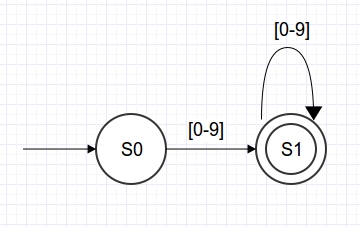
\includegraphics[width=0.7\textwidth]{../0-lexico/automatos/integer}
\end{figure}

\begin{figure}[H]
  \caption{Automato que reconhece um número real}
  \centering
    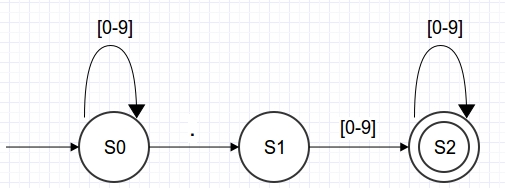
\includegraphics[width=0.7\textwidth]{../0-lexico/automatos/float}
\end{figure}

\begin{figure}[H]
  \caption{Automato que reconhece um identificador}
  \centering
    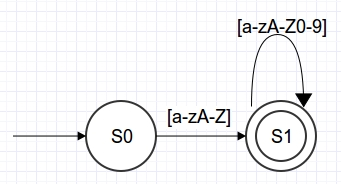
\includegraphics[width=0.7\textwidth]{../0-lexico/automatos/keyword_identifier}
\end{figure}

\begin{figure}[H]
  \caption{Automato que reconhece um caracter}
  \centering
    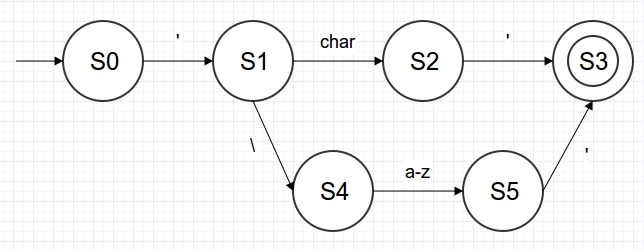
\includegraphics[width=0.7\textwidth]{../0-lexico/automatos/char}
\end{figure}

\begin{figure}[H]
  \caption{Automato que reconhece uma cadeia de caractéres}
  \centering
    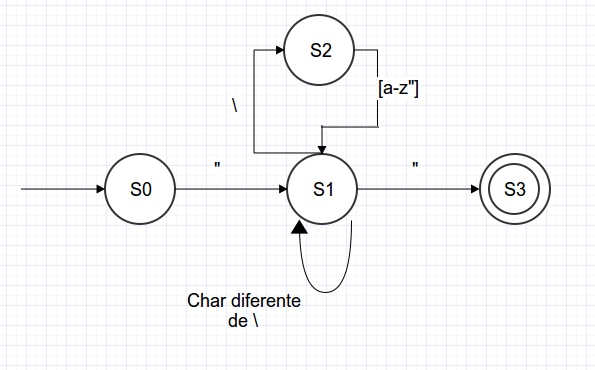
\includegraphics[width=0.7\textwidth]{../0-lexico/automatos/string}
\end{figure}

\begin{figure}[H]
  \caption{Automato que reconhece operadores}
  \centering
    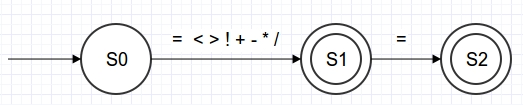
\includegraphics[width=0.7\textwidth]{../0-lexico/automatos/operators}
\end{figure}

\begin{figure}[H]
  \caption{Automato que reconhece delimitadores}
  \centering
    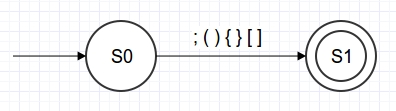
\includegraphics[width=0.7\textwidth]{../0-lexico/automatos/delimiters}
\end{figure}

\begin{figure}[H]
  \caption{Automato que reconhece comentários e caractéres ignorados}
  \centering
    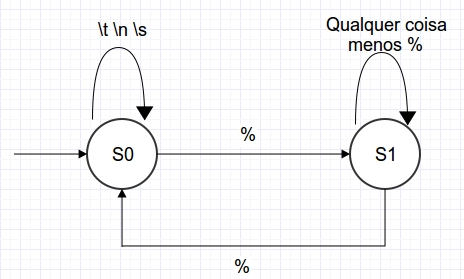
\includegraphics[width=0.7\textwidth]{../0-lexico/automatos/non-used}
\end{figure}

\section{Questão 5}

\textbf{Crie um autômato único que aceite todas essas linguagens a partir de um mesmo estado inicial, mas que apresente um estado final diferenciado para cada uma delas}

\begin{figure}[H]
  \caption{Automato completo}
  \centering
    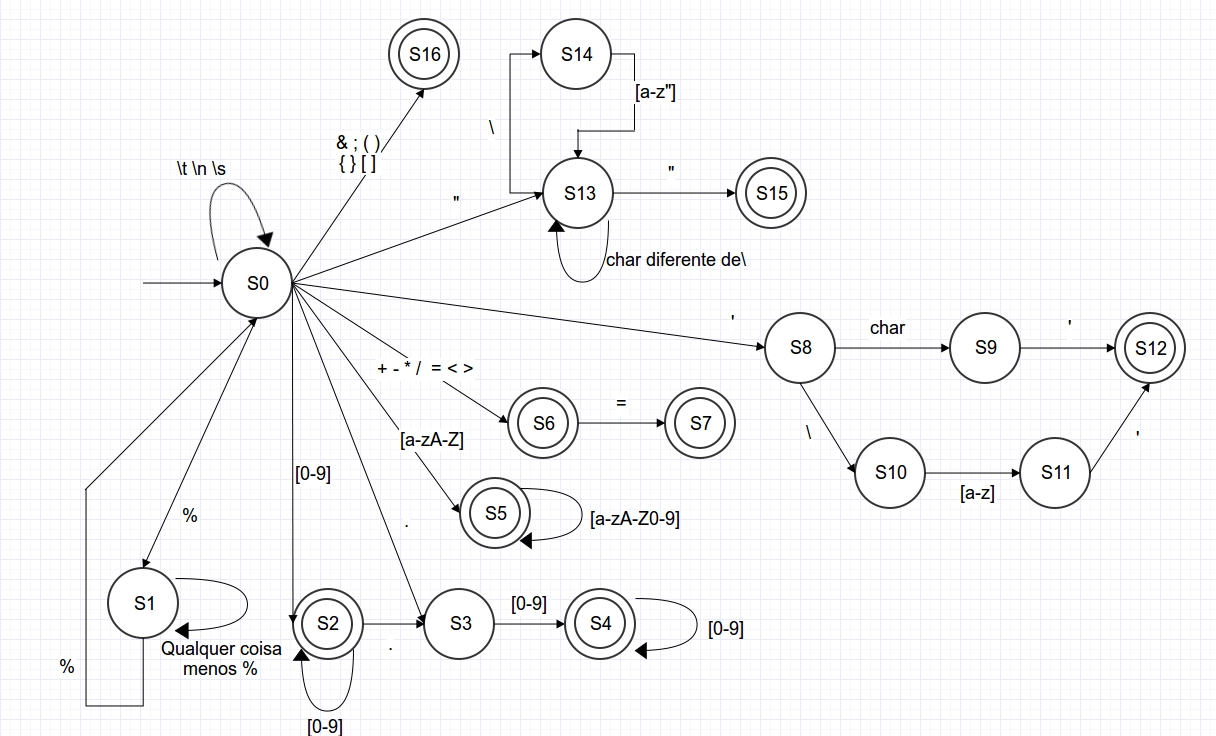
\includegraphics[width=\textwidth]{../0-lexico/automatos/completo}
\end{figure}

\section{Questão 6}

\textbf{Transforme o autômato assim obtido em um transdutor, que emita como saída o átomo encontrado ao abandonar cada um dos estados finais para iniciar o reconhecimento de mais um átomo do texto}

Idem ao item anterior. A diferença é que haverá $\epsilon$-transições adicionais partindo dos estados de aceitação, dando como saída o token, e tendo como destino o estado inicial da máquina S0.

\section{Funcionamento do Módulo de Análise Léxica}

\begin{figure}[H]
  \caption{Arquitetura do analisador léxico}
  \centering
    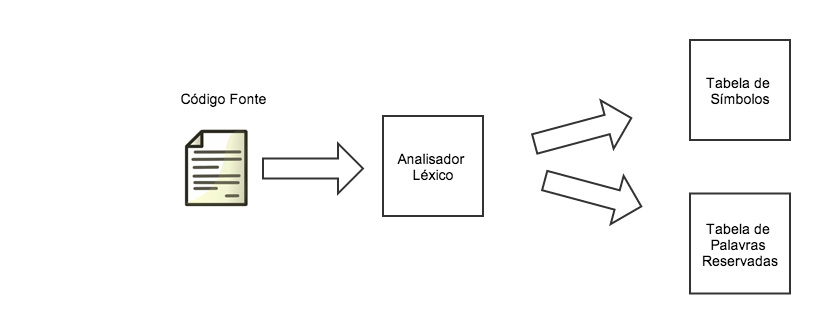
\includegraphics[width=0.7\textwidth]{../0-lexico/automatos/lexical_analyzer}
\end{figure}

Basicamente, o analisador léxico pode ser visto como um sistema composto por quatro módulos.

\subsection{Tabela de palavras reservadas}

Implementamos esse módulo como sendo o responsável pela leitura de um arquivo externo o qual contém as palavras reservadas consideradas pela linguagem do compilador e pela poulação de uma estrutura de dados (no nosso caso, uma lista ligada - /linked\_list/linked\_list.c) que será consultada pelo leitor de expressões regulares de forma a identificar as palavras reservadas.

A ideia de utilizar um arquivo externo é ter uma visão de evolução potencial da linguagem, caso novas palavras reservadas passem a fazer parte da linguagem ou caso antigas palavras sejam removidas/modificadas. Nesse arquivo há uma palavra reservada por linha. O arquivo atual de entrada se chama keywords e está localizado na pasta context\_stack.

Este módulo foi implementado no arquivo keyword\_analyser.c dentro da pasta context\_stack.

\subsection{Tabela de símbolos}

O módulo da tabela de simbolos é composto do arquivo symbol\_table.c dentro da pasta context\_stack.

Ele também utiliza a estrura de dados (lista ligada), no qual cada nó contém uma estrura do tipo:

\lstset{language=C}
\begin{lstlisting}[frame=single]
typedef struct{
    char* id;
    int value;
    Type type;
} Symbol;
\end{lstlisting}

Uma das principais funcionalidades fornecidas por este módulo ao analisador léxico é a possibilidade de inserir novos símbolos à tabela. A inserção de identificadores é única na tabela.
Ele também permite, em um segundo momento, a sua consulta pelo analisador sintático.

\subsection{Tabela de transições}

Consiste em um arquivo externo que modela uma máquina de estados, resultante do transdutor dos exercícios anteriores. 
O arquivo /lexical\_analyser/lex\_machine contém:

\begin{itemize}
	\item Primeira linha: número n de estados total da máquina
	\item Segunda linha: número m de estados de aceitação
	\item Próximas m linhas: identificador do estado (int) seguido de seu nome (char[3]) - o mesmo nome será utilizado para identificação do token retornado pelo estado
	\item Próxima linha: número k de estados que serão ignorados pelo módulo (comentário, espaços em branco etc.)
	\item Próximas k linhas: identificadores dos estados ignorados
	\item Próximas n linhas: representação da tabela de transições. Cada linha representa um estado $\sigma_n$ e cada coluna um caracter de entrada $a$. Os valores das células representam o $f(\sigma_n, a)$.
\end{itemize}

Nota: transições resultando em -1 indicam um estado de saída - a máquina pára, indicando ao leitor de expressões regulares que foi encontrado :

\begin{itemize}
	\item uma das expressões regulares definidas pela gramática da linguagem 
	\item um erro
	\item uma expressão ignorada (comentário, espaços em branco etc.)
\end{itemize}

Em seguida, a máquina realiza uma $\epsilon$-transição para o estado inicial S0.

\subsection{Leitor de expressões regulares}

O módulo de leitura de expressões regulares é o módulo central que integra e controla o fluxo de dados dos outros três módulos periféricos. Seu modo de operação obdece à seguinte rotina:

\begin{itemize}
	\item init\_lex:

	\begin{enumerate}
		\item inicializa a máquina de estados, a partir da Tabela de transições
		\item inicializa a Tabela de Palavras Reservadas
		\item inicializa em branco a Tabela de Símbolos
	\end{enumerate}

	\item get\_token: lê o código fonte e usa a máquina de estados inicializada anteriormente para tentar encontrar uma das expressões regulares definidas pela gramática. Quando a máquina pára, é realizada a leitura do buffer para gerar um token (classe, valor e posição no arquivo fonte). Caso a máquina tenha parado no estado que indica a expressão regular de um identificador, fazemos uma consulta à Tabela de Palavras Reservadas. E se for o caso deste ser uma palavra reservada, mudamos sua classe de identificador para palavra reservada (KEY). Caso contrário, inserimos o identificador na Tabela de Símbolos e o consideramos como sendo da classe de variáreis (VAR).
\end{itemize}

\subsection{Programa Principal}

O programa principal chama repetidamente a sub-rotina get\_token() do analisador léxico sobre um arquivo do tipo texto contendo o texto-fonte a ser analisado. Após cada chamada, esse programa principal imprimi o conteúdo do token. O programa termina ao receber um token especial (EOA), o qual indica o fim do arquivo; ou ao receber um token de erro. 


\section{Descrição dos testes realizados e das saídas obtidas}

O teste foi realizado, utilizando o próprio código em cópia do arquivo fonte do analisador léxico (ENTRADA.txt), mais especificamente a função main.
Na saída deste teste (SAIDA.txt), obtemos:
A Tabela de Palavras Reservadas
Os tokens retornados pela chamada recorrente da subrotina get\_token()
Finalmente a Tabela de Símbolos resultante da leitura da entrada (somente os nomes dos identificadores) 

A saída efetiva foi igual à saída esperada.

\section{Questão 10}
\textbf{Explique como enriquecer esse analisador léxico com um expansor de macros do tipo \#DEFINE, não paramétrico nem recursivo, mas que permita a qualquer macro chamar outras macros, de forma não cíclica. (O expansor de macros não precisa ser implementado)} 

Baseando-se na método de como C implementa macros, o analisador léxico poderia usar de um pré-compilador que gera um código intermediário com as macros expandidas. O pré-compilador percorreria o código original, procurando a existência de macros e expandiria essas macros, salvando o resultado em um código intermediário. O pré-compilador continuaria a iterar o código intermediário na busca de macros, as expandindo, até que não exista mais macros no código. Código intermediário resultante seria então passado para o léxico para ser feita a análise léxica.

Implementando as macros dentro do próprio léxico, o analisador poderia usar uma pilha de buffers. Ao encontrar uma macro, o léxico carregaria a macro em um buffer, pararia a execução do arquivo/buffer que ele está lendo atualmente e empilharia o novo buffer na pilha. Esse novo buffer seria a nova fonte de dados para léxico, até que o buffer fosse terminado. Ele é então desempilhado, e o próximo topo da pilha será a nova fonte.
